\documentclass[11pt,oneside]{scrbook}
\usepackage[a4paper,margin=2.4cm,marginparwidth=1.8cm,marginparsep=0.4cm]{geometry}
\usepackage{../common/rlstudy}
\usepackage[ruled,vlined]{algorithm2e}
\newcommand{\Reg}{\mathrm{Reg}}
\newcommand{\PUCT}{\mathrm{PUCT}}

\title{{\color{rlblue}\textbf{Week 13} \\ \Huge Multi-Agent RL and AlphaZero}}
\author{STUDY-RL --- a self-paced Deep RL curriculum}
\date{\today}

\begin{document}
\maketitle
\tableofcontents
\newpage

% =============================================================================
\chapter*{Learning objectives}
\addcontentsline{toc}{chapter}{Learning objectives}


% Teaching companion: a small example before the full lecture.
\noindent\textbf{Study companion.} Read \texttt{teaching\_guide.md} in this
folder for step-by-step examples, an analogy with its limits, and self-checks.
Then use \texttt{workbook.ipynb} to implement and vary the calculations.
\par\medskip

\begin{keyidea}
By the end of this lecture you will be able to:
\begin{enumerate}\setlength\itemsep{2pt}
  \item Distinguish cooperative, competitive, and mixed multi-agent settings;
        state the centralised-training / decentralised-execution (CTDE)
        paradigm.
  \item Derive the policy gradient for MADDPG and the centralised critic of
        MAPPO; explain why CTDE works even when the execution-time policy is
        decentralised.
  \item State and discuss the QMIX monotonicity caveat: when does the
        factorised joint Q-function approximate the true joint Q-function?
  \item Explain self-play, fictitious play, and Policy-Space Response
        Oracles (PSRO) as iterative best-response procedures.
  \item Derive the AlphaZero MCTS-with-PUCT selection rule, the
        Dirichlet-noise exploration scheme, and the joint policy/value
        training loss.
  \item Train a small AlphaZero on Tic-Tac-Toe (3x3) to near-optimal play
        in $\sim 1$ minute on CPU; observe the ELO-style winrate climb.
  \item Train MAPPO on a coordination matrix game to perfect coordination,
        and on a SimpleSpread-style cooperative-coverage env (noisy but
        non-trivial).
\end{enumerate}
\end{keyidea}

% =============================================================================
\chapter{Motivation and intuition}

The single-agent RL we have built so far assumes the environment is
stationary --- the transition dynamics do not change. In multi-agent
settings this is false: each other agent's policy is part of the
environment, and as other agents learn, the environment shifts under you.
This is the \emph{non-stationarity problem} of MARL.

Multi-agent problems come in three flavours:

\textbf{Cooperative.} All agents share a reward signal. Examples:
ride-hailing dispatch, factory floor coordination, multi-robot search.
The algorithmic challenge is credit assignment (who contributed to the
shared reward) and coordination (without explicit communication, how do
agents converge on compatible policies). \emph{This is what MAPPO solves.}

\textbf{Competitive.} Zero-sum: one agent's gain is another's loss. The
canonical examples are board games (chess, go, poker) and adversarial
robust-RL (one agent picks dynamics, the other picks policies). The
algorithmic challenge is the moving-target problem: as opponent improves,
the policy that beat the old opponent loses to the new one.
\emph{This is what AlphaZero solves.}

\textbf{Mixed (general-sum).} Some shared, some opposed interests. Two-sided
matching markets (synthetic insurance brokers vs.\ leads, ATS recruiters vs.\
candidates) fall here: the platform's reward is system-level binds /
hires; each broker / candidate has private preferences and may game the
allocator. The algorithmic question is \emph{equilibrium selection}: which
Nash equilibrium does the multi-agent learning dynamics converge to, and
is it a desirable one?

\section{Anchoring}

You already know self-play if you have ever trained a GAN: the generator
and discriminator are two agents in a zero-sum game, each adapting to the
other's current best policy. AlphaZero is GAN-with-MCTS: the policy is the
generator, the value head is the discriminator, MCTS is the adversarial
optimisation that picks the next move.

You already know MAPPO if you know PPO: it is PPO with a centralised critic
that consumes the global state and per-agent actors that consume only
local observations. Centralised critic, decentralised execution --- the
critic at training time sees everything, but at deployment each agent
acts on local information alone.

\section{Why this week sits where it does}

Bandits (Week 11) and ranking (Week 12) are degenerate one-step games.
This week we put the games back. The same machinery (UCB, posterior
sampling, importance-weighted policy gradients) carries over with the
extension that each agent's update must anticipate the others' updates.
Self-play and PSRO are best-response \emph{cascades}: I update my best
response to your current policy, you update yours, repeat. Provably
convergent in two-player zero-sum games; messier in general-sum.

\begin{pitfall}
The non-stationarity problem is the central pitfall of MARL. A naive
extension of single-agent DQN to two agents (each running independent DQN)
loses every theoretical convergence guarantee. Empirically it sometimes
works, often does not. CTDE was invented to recover stability: the
centralised critic provides a stationary learning signal.
\end{pitfall}

% =============================================================================
\chapter{Mathematical formulation}

\section{Stochastic games}

\begin{definition}[Stochastic game / Markov game]
A tuple $(N, \mathcal{S}, \{\mathcal{A}_i\}_{i=1}^N, P, \{r_i\}_{i=1}^N, \gamma)$.
$N$ agents act simultaneously in shared state $s_t$; the joint action
$\mathbf{a}_t = (a_{1,t}, \dots, a_{N,t})$ determines the next state
$s_{t+1} \sim P(\cdot | s_t, \mathbf{a}_t)$ and reward
$r_{i,t} \sim r_i(s_t, \mathbf{a}_t)$ for each agent.
\end{definition}

Special cases:
\begin{itemize}\setlength\itemsep{1pt}
  \item \emph{Cooperative}: $r_i \equiv r$ for all $i$.
  \item \emph{Zero-sum 2-player}: $r_1 + r_2 \equiv 0$.
  \item \emph{General-sum}: no constraints.
  \item \emph{Dec-POMDP}: cooperative + partial observability (each agent
        only sees $o_i$, not $s$).
\end{itemize}

\begin{definition}[Nash equilibrium]
A joint policy $\boldsymbol{\pi}^\star = (\pi_1^\star, \dots, \pi_N^\star)$ is
a Nash equilibrium if for every agent $i$ and every alternative policy
$\pi_i'$,
\[
V_i^{\boldsymbol{\pi}^\star} \;\geq\; V_i^{(\pi_i', \boldsymbol{\pi}_{-i}^\star)}.
\]
No agent can unilaterally improve by deviating.
\end{definition}

\begin{intuition}
Nash is the right solution concept when agents are strategic. In
cooperative settings it is overkill (the optimal joint policy is a Nash
but so is every coordination failure); in zero-sum it is tight (the
minimax value). General-sum may have multiple Nashes and learning may
oscillate among them.
\end{intuition}

\section{Cooperative MARL: centralised critic, decentralised execution}

The CTDE recipe:
\begin{itemize}\setlength\itemsep{1pt}
  \item Each agent $i$ has a \emph{decentralised actor} $\pi_i(a_i \mid o_i, \theta_i)$
        with parameters $\theta_i$ that depends only on its local observation.
  \item A \emph{centralised critic} $V(s; \phi)$ or $Q(s, \mathbf{a}; \phi)$
        consumes the global state (and possibly all agents' actions) and
        is used \emph{only at training time}.
  \item At deployment, each agent runs only its decentralised actor; the
        critic is discarded.
\end{itemize}

The advantage of CTDE: the critic sees through the non-stationarity (it
has all agents' actions as input, so the joint dynamics are Markov in its
input space) while the deployed system remains decentralised (no shared
network at inference time).

\subsection{MADDPG (Lowe et al.\ NeurIPS 2017)}

The first CTDE-style continuous-action algorithm. Per-agent deterministic
policy $a_i = \mu_i(o_i; \theta_i)$, per-agent centralised critic
$Q_i(s, \mathbf{a}; \phi_i)$ trained on the multi-agent Bellman:

\begin{theorem}[MADDPG policy gradient, Lowe et al.\ 2017]
The deterministic policy gradient for agent $i$ is
\[
\nabla_{\theta_i} J(\mu_i) = \E_{s \sim D}\Big[\nabla_{\theta_i} \mu_i(o_i) \nabla_{a_i} Q_i(s, \mathbf{a})\big|_{a_i = \mu_i(o_i)}\Big].
\]
\end{theorem}

\begin{proof}[Sketch]
The single-agent DDPG result generalises directly: the deterministic
policy gradient is the inner product of the policy's Jacobian with the
critic's gradient. The only change in MARL is that the critic depends
on $\mathbf{a}_{-i}$ (other agents' actions), which are not differentiated
through. $\square$
\end{proof}

\subsection{MAPPO (Yu et al.\ NeurIPS 2022)}

A simple but powerful recipe: vanilla PPO, but with a centralised
state-value critic. Per-agent actor takes $o_i$, the critic takes the
global state $s$. The PPO objective is unchanged per agent:
\[
L^{\mathrm{CLIP}}_i(\theta_i) = \E\Big[\min\big(r_t(\theta_i) A_t^{\mathrm{GAE}}, \mathrm{clip}(r_t(\theta_i), 1-\epsilon, 1+\epsilon) A_t^{\mathrm{GAE}}\big)\Big].
\]
The advantage $A_t^{\mathrm{GAE}}$ is computed from the centralised value
function. The critic is shared across agents (one network, fed each
agent's transitions); the actor is per-agent (or can be shared too, with
agent-id embedding).

\begin{theorem}[MAPPO surprise, Yu et al.\ NeurIPS 2022]
With careful normalisation and centralised value functions, MAPPO matches
or exceeds MADDPG, QMIX, COMA, and IPPO on the StarCraft Multi-Agent
Challenge (SMAC) and the Multi-Agent MuJoCo benchmark, despite being one
of the simplest CTDE recipes.
\end{theorem}

\subsection{QMIX (Rashid et al.\ ICML 2018)}

Value-decomposition: factorise $Q_{\mathrm{joint}}(s, \mathbf{a}) = f(Q_1(o_1, a_1), \dots, Q_N(o_N, a_N))$
where $f$ is a monotone aggregator (a mixing network with non-negative
weights). This makes \emph{decentralised greedy decisions consistent with
joint argmax}:
\[
\argmax_{\mathbf{a}} Q_{\mathrm{joint}}(s, \mathbf{a}) = (\argmax_{a_1} Q_1, \dots, \argmax_{a_N} Q_N).
\]

\begin{remark}[QMIX monotonicity caveat]
The monotone aggregator is a strict restriction: it cannot represent joint
Q-functions where one agent's best action depends on another agent's
action in a way that flips ordering (the canonical counter-example is a
``XOR-coordination'' game). For tasks like SimpleSpread / SMAC where
optimal play has compatible per-agent argmax actions, QMIX works; for
adversarial-coordination tasks, it fails.
\end{remark}

\section{Competitive MARL: self-play, fictitious play, PSRO}

\subsection{Self-play}

Both agents share the same policy network; each is trained against
opponents that are previous versions of the same network. Goes back to
Tesauro's TD-Gammon (1992) and is the recipe behind AlphaGo, AlphaZero,
AlphaStar, and OpenAI Five.

\begin{theorem}[Self-play convergence in zero-sum games, Singh et al.\ 2000]
In a two-player zero-sum stochastic game, fictitious-play self-play
converges to the minimax (Nash) equilibrium under standard regularity
conditions. The result extends to function-approximation settings under
the additional assumption that the function class realises the
equilibrium.
\end{theorem}

\subsection{Fictitious play}

At iteration $t$, each agent plays the best response to the empirical
distribution of the opponent's historical actions $\bar\pi_{-i}^{(t)} = \frac{1}{t} \sum_{k=1}^t \pi_{-i}^{(k)}$.
In matrix games this is guaranteed to converge to a Nash equilibrium in
zero-sum and identical-interest games (Robinson 1951; Monderer \&
Shapley 1996).

\subsection{Policy-Space Response Oracles (PSRO)}

\begin{definition}[PSRO, Lanctot et al.\ NeurIPS 2017]
Iterate: (i) compute a Nash equilibrium $\sigma^{(t)}$ on the current
population of policies $\Pi^{(t)}$; (ii) for each agent, compute the best
response to $\sigma^{(t)}_{-i}$ via single-agent RL; (iii) add the best
responses to the population; repeat.
\end{definition}

PSRO unifies self-play, fictitious play, and double-oracle algorithms. The
inner ``best response'' step is the only RL step; the meta-game over the
policy population is solved by classical game-theoretic methods (LP for
zero-sum, replicator dynamics for general-sum).

\begin{theorem}[PSRO convergence in two-player zero-sum games, Lanctot et al.\ 2017]
In a two-player zero-sum game, PSRO converges to an $\epsilon$-Nash
equilibrium in finite iterations under exact best response. With
approximate best response (PPO with bounded sample complexity), the
convergence rate degrades to $\tilde O(1/\sqrt{T})$.
\end{theorem}

% =============================================================================
\chapter{AlphaZero}

This chapter is the heart of the lecture. AlphaZero (Silver et al.\
\emph{Mastering Chess and Shogi by Self-Play with a General Reinforcement
Learning Algorithm}, Science 2018; \emph{Mastering the game of Go without
human knowledge}, Nature 2017) unifies MCTS, deep RL, and self-play into
a single training loop that has produced super-human play in Go, Chess,
Shogi, and (with extensions like MuZero) Atari.

\section{The core idea}

AlphaZero has three components:

\textbf{(1) A policy/value network.} A single network with two heads:
$\pi(\cdot \mid s; \theta) \in \Delta(\Actions)$ predicts a policy
distribution; $v(s; \theta) \in [-1, 1]$ predicts the expected outcome from
$s$.

\textbf{(2) Monte Carlo Tree Search.} Given a root state, MCTS uses the
network as a heuristic to do focused tree search. Output: a refined policy
$\pi_{\mathrm{MCTS}}(\cdot \mid s)$ that is provably better than the raw
network policy (proof: MCTS visits the best moves more, so the visit-count
distribution is a strict improvement).

\textbf{(3) Self-play training.} Generate games by self-play using MCTS at
each move. For each (state, $\pi_{\mathrm{MCTS}}$, game-result) triple,
train the network to predict $\pi_{\mathrm{MCTS}}$ from the policy head
and the game-result from the value head:
\[
\mathcal{L}(\theta) = -\sum_a \pi_{\mathrm{MCTS}}(a) \log \pi(a \mid s; \theta) + (v(s; \theta) - z)^2 + \mathrm{wd}(\theta).
\]

The training loop is a self-improvement cascade: better network produces
better MCTS produces better self-play data produces a better network.

\section{MCTS with PUCT}

\begin{definition}[PUCT selection rule, Silver et al.\ 2017]
At each node $n$ with children $c$, select the child $c^\star$ maximising
\[
\PUCT(n, c) \;=\; -Q(c) \;+\; c_{\mathrm{puct}}\, P(c) \cdot \frac{\sqrt{N(n)}}{1 + N(c)},
\]
where $Q(c)$ is the mean action-value from previous simulations (negated
because the child's $Q$ is from the opponent's perspective), $P(c)$ is the
prior probability from the policy network, $N(n)$ is the parent's visit
count, $N(c)$ is the child's visit count, and $c_{\mathrm{puct}}$ is an
exploration constant (typically $1$--$4$).
\end{definition}

\begin{intuition}
PUCT is UCB1 with two changes: (1) the bonus uses the \emph{prior policy}
as a multiplier (so the network's preferences guide exploration), and (2)
the bonus shrinks as $\sqrt{N(n)} / (1 + N(c))$ instead of
$\sqrt{\log N / N(c)}$. The $\sqrt{N}$ in the numerator (rather than
$\sqrt{\log N}$) gives \emph{aggressive} exploration of the priors;
empirically this is what makes AlphaZero work on board games.
\end{intuition}

\begin{theorem}[PUCT regret on bandit subproblems, Rosin 2011]
On the bandit subproblem at any tree node, PUCT achieves
$O(\sqrt{N \log K})$ regret asymptotically, matching the minimax-optimal
rate for $K$-armed bandits with strong priors.
\end{theorem}

\section{Dirichlet noise}

At the root of every MCTS, AlphaZero adds Dirichlet noise to the prior:
\[
P'(\cdot \mid s_{\mathrm{root}}) = (1 - \epsilon) P(\cdot \mid s_{\mathrm{root}}) + \epsilon\, \eta, \quad \eta \sim \mathrm{Dirichlet}(\alpha \mathbf{1}).
\]
Typical values: $\epsilon = 0.25$, $\alpha = 0.3$ for Go, $\alpha = 0.5$
for chess. The noise injects exploration at the root, preventing the
network from collapsing onto a single move.

\begin{pitfall}
Forgetting the Dirichlet noise is the most common AlphaZero bug. Without
it, the policy network gets trained only on its own preferences, never
explores alternatives, and converges to a sub-optimal fixed point. The
noise is the only source of exploration in the entire pipeline.
\end{pitfall}

\section{Training loss}

\begin{theorem}[AlphaZero training loss]
For each self-play tuple $(s, \pi_{\mathrm{MCTS}}, z)$, the loss is
\[
\mathcal{L}(\theta; s, \pi_{\mathrm{MCTS}}, z) = (z - v(s; \theta))^2 - \pi_{\mathrm{MCTS}}^\top \log \pi(\cdot \mid s; \theta) + c \|\theta\|^2.
\]
The first term regresses the value head to the game outcome; the second
trains the policy head to match the MCTS visit distribution; the third is
L2 regularisation.
\end{theorem}

\begin{proof}[Why this works]
The MCTS visit distribution $\pi_{\mathrm{MCTS}}$ is a \emph{policy
improvement} over the network's raw $\pi(\cdot \mid s; \theta)$ because MCTS
visits high-value actions more (the bandit subproblem at each node has
sub-linear regret on the visit distribution). So training the network to
match $\pi_{\mathrm{MCTS}}$ improves the network's policy. Similarly, the
game outcome $z$ is an unbiased sample of $V^\pi(s)$ under the current
self-play policy, so the value head learns the current policy's value
function. The combination is a generalised-policy-iteration step: improve
the policy, evaluate the policy, repeat. $\square$
\end{proof}

\section{Symmetry augmentation}

For Tic-Tac-Toe (and Go, and chess to a lesser extent), the game has
geometric symmetries. AlphaZero augments each (state, $\pi_{\mathrm{MCTS}}$,
$z$) tuple with all $D_4$ symmetries (4 rotations $\times$ 2 reflections =
8 augmentations on a square board). This multiplies the effective dataset
by 8 at no compute cost and is essential for fast learning on small boards.

\section{Putting it together}

\begin{algorithm}[H]
\caption{AlphaZero training loop}\label{alg:az}
\DontPrintSemicolon
\KwIn{Network $f_\theta = (\pi, v)$, MCTS budget $n_{\mathrm{sim}}$, exploration constant $c_{\mathrm{puct}}$, Dirichlet $(\epsilon, \alpha)$.}
\textbf{Init:} Replay buffer $\mathcal{D} = \emptyset$.\;
\For{iteration $= 1, 2, \dots$}{
  \For{self-play episode}{
    $s \leftarrow$ initial state\;
    \While{$s$ is non-terminal}{
      Run MCTS with $f_\theta$ from $s$ for $n_{\mathrm{sim}}$ simulations (with Dirichlet noise at root).\;
      $\pi_{\mathrm{MCTS}} \leftarrow$ normalised visit counts at root.\;
      Sample $a \sim \pi_{\mathrm{MCTS}}^{1/\tau}$ (with temperature $\tau$).\;
      For each symmetry $g$, store $(g \cdot s, g \cdot \pi_{\mathrm{MCTS}})$ in $\mathcal{D}$.\;
      $s \leftarrow s'$ after applying $a$.\;
    }
    For each stored tuple in this episode, set $z$ = game result from the player's perspective.\;
  }
  \For{training epoch}{
    Sample minibatch from $\mathcal{D}$.\;
    Take SGD step on $\mathcal{L}(\theta; s, \pi_{\mathrm{MCTS}}, z)$.\;
  }
  Evaluate $f_\theta$ vs.\ previous best; if winrate $>$ threshold, replace.\;
}
\end{algorithm}

% =============================================================================
\chapter{MuZero, MCTS extensions, and modern self-play}

\section{MuZero (Schrittwieser et al.\ Nature 2020)}

The natural extension of AlphaZero to environments where the dynamics are
unknown. MuZero learns a latent dynamics model alongside the policy and
value: at each MCTS expansion, instead of applying the true environment
transition, the network predicts a latent next-state and a reward. The
tree search happens entirely in the latent space.

\begin{theorem}[MuZero loss]
Joint loss across $K$-step unrolls:
\[
\mathcal{L} = \sum_{k=0}^K \big[\ell^p(\pi_k^{\mathrm{MCTS}}, \pi_k) + \ell^v(z_k, v_k) + \ell^r(u_k, r_k)\big] + c \|\theta\|^2,
\]
where $\ell^r$ is the model's reward-prediction loss and $u_k$ is the
observed reward at unroll step $k$.
\end{theorem}

\textbf{Why MuZero matters.} It unifies AlphaZero (board games) and
Atari-style RL (no model) into a single framework. The latent dynamics
model is trained \emph{end-to-end with the policy and value}, so it learns
exactly the features that matter for planning. MuZero achieves
super-human play in Go / Chess / Shogi \emph{and} sets new SOTA on Atari
with the same algorithm.

\section{Stochastic MuZero and EfficientZero}

\textbf{Stochastic MuZero} (Antonoglou et al.\ 2022) extends to stochastic
environments by sampling latent next-states. \textbf{EfficientZero}
(Ye et al.\ NeurIPS 2021) adds a self-supervised consistency loss between
predicted and actual next states, plus a search-policy entropy bonus;
trains to near-MuZero Atari scores with $\sim 1/100$ the data.

\section{KataGo and the AlphaZero hyperparameter zoo}

KataGo (Wu 2019, ongoing) is the open-source Go engine descended from
AlphaGo Zero. It has spent five years optimising the AlphaZero recipe:
playout cap randomisation (small-search games for fast iteration,
big-search games for label quality), targeted exploration of
unbalanced positions, score-based auxiliary heads, transfer learning
across board sizes. The net effect: KataGo at $\sim 10^4$ TPU-hours
matches AlphaGo Zero at $\sim 10^6$ TPU-hours. The lessons:
\begin{itemize}\setlength\itemsep{1pt}
  \item Mixing playout budgets across self-play games is a free win
        (Wu 2019); some games with 50 sims, some with 1000.
  \item Auxiliary heads (score, ownership, ranking) regularise the
        backbone and stabilise the policy / value heads.
  \item Symmetry augmentation is essential at small sizes (we exploit
        the same on Tic-Tac-Toe).
\end{itemize}

\section{Self-play in two-player zero-sum games: theory}

\begin{theorem}[Self-play converges to Nash, Singh, Kearns, Mansour 2000]
In a two-player zero-sum stochastic game, if both players use
no-regret learning algorithms (e.g., Hedge / Exp3), the time-average
of joint policies converges to a Nash equilibrium.
\end{theorem}

The result generalises to extensive-form games via Counterfactual Regret
Minimisation (CFR; Zinkevich et al.\ NeurIPS 2007), which is the
algorithm behind the super-human poker bots Libratus (Brown \& Sandholm
Science 2017) and Pluribus (Brown \& Sandholm Science 2019).

\section{League training (AlphaStar)}

AlphaStar (Vinyals et al.\ Nature 2019) extends self-play to handle
\emph{non-transitive} games (StarCraft II, where rock-paper-scissors
dynamics exist between unit compositions). The recipe:
\begin{itemize}\setlength\itemsep{1pt}
  \item Maintain a \emph{league} of past policies.
  \item Train ``main agents'' against the league with a prioritised
        sampling that focuses on the league's strongest exploiters.
  \item Periodically add the main agent's snapshot back to the league.
  \item Train ``main exploiters'' (focused on beating main agents) and
        ``league exploiters'' (focused on beating the league average).
\end{itemize}
This produces robust play against the entire StarCraft strategy space ---
not just whatever the latest opponent happened to play.

% =============================================================================
\chapter{Algorithms}

\begin{algorithm}[H]
\caption{MAPPO with centralised critic}\label{alg:mappo}
\DontPrintSemicolon
\KwIn{$N$ agents, per-agent actor $\pi_i(a_i | o_i; \theta_i)$, centralised critic $V(s; \phi)$, PPO clip $\epsilon$.}
\For{iteration $= 1, 2, \dots$}{
  \tcp{Rollout}
  \For{episode}{
    \For{$t = 1, \dots, T$}{
      Each agent $i$ samples $a_{i,t} \sim \pi_i(\cdot \mid o_{i,t})$.\;
      Step env: $s_{t+1}, \{r_{i,t}\} \leftarrow \mathrm{env}.\mathrm{step}(\mathbf{a}_t)$.\;
      Store $(o_{i,t}, a_{i,t}, \log \pi_i(a_{i,t} | o_{i,t}), r_{i,t}, V(s_t), s_t)$.\;
    }
  }
  \tcp{GAE per agent}
  \For{agent $i = 1, \dots, N$}{
    Compute $A^{\mathrm{GAE}}_{i,t}$ from $(r_{i,t}, V(s_t))$.\;
  }
  \tcp{PPO update}
  \For{epoch $= 1, \dots, K$}{
    Sample minibatch; compute $L^{\mathrm{CLIP}}_i$ and critic MSE.\;
    Step on $\sum_i L^{\mathrm{CLIP}}_i + \tfrac{1}{2}(V(s) - R)^2$.\;
  }
}
\end{algorithm}

\begin{algorithm}[H]
\caption{Self-play in zero-sum games}\label{alg:sp}
\DontPrintSemicolon
\KwIn{Initial policy $\pi^{(0)}$, training procedure $\mathrm{Train}(\cdot, \cdot)$.}
\For{iteration $t = 1, 2, \dots$}{
  Sample games with $\pi^{(t-1)}$ playing both sides.\;
  $\pi^{(t)} \leftarrow \mathrm{Train}(\pi^{(t-1)}, \mathrm{games}_t)$.\;
  Evaluate $\pi^{(t)}$ vs.\ a fixed test opponent; track ELO climb.\;
}
\end{algorithm}

\begin{example}[A by-hand MCTS rollout on Tic-Tac-Toe]
Initial state (all empty), to-move = X. Suppose the network priors put
$P(\text{centre}) = 0.5$, $P(\text{corner}) = 0.1$ each (4 corners),
$P(\text{edge}) = 0.025$ each (4 edges). $c_{\mathrm{puct}} = 1.5$.

\textbf{Simulation 1.} Root has $N = 0$; PUCT bonus is
$1.5 \cdot P(c) \cdot \sqrt{0}/(1+0) = 0$ for all children --- the
selection rule degenerates to ``pick by prior''. Centre wins: $a = \text{centre}$. Network
evaluates the resulting state (one X in centre, O to move); say
$v = -0.1$ (slight advantage to X from X's POV). Backpropagate: root's
centre child gets $Q = 0.1$, $N = 1$.

\textbf{Simulation 2.} Root's centre child has $Q = -0.1$ from O's POV;
its PUCT score from root is $-(-0.1) + 1.5 \cdot 0.5 \cdot \sqrt{1}/(1+1) = 0.475$.
Each corner has $Q = 0$ and PUCT $= 0 + 1.5 \cdot 0.1 \cdot 1/1 = 0.15$.
Centre wins again; we expand a child move (say corner from O's POV).
Network gives value $v = -0.05$.

After 30 simulations, centre typically has $\sim$15 visits, corners
$\sim$3 each, edges $\sim$1 each. The output $\pi_{\mathrm{MCTS}}$ is
$\approx (0.5, 0.1, 0.1, 0.1, 0.1, 0.03, 0.03, 0.02, 0.02)$ depending on
final visit counts. This $\pi_{\mathrm{MCTS}}$ is what trains the policy
network on the next iteration.
\end{example}

\textbf{Complexity.} MCTS per move: $O(n_{\mathrm{sim}} \cdot \text{depth})$
network evaluations. For 30 simulations on Tic-Tac-Toe (max depth 9), this
is $\sim 200$ evaluations per move, $\sim 1000$ per game. Self-play of $\sim 1000$
games per iteration is $\sim 10^6$ evaluations --- about 1 minute on CPU.
MAPPO scales linearly in number of agents (per-agent actor inference) and
linearly in episode length.

\begin{pitfall}
The number of MCTS simulations is the single most important hyperparameter
in AlphaZero. Too few and the policy improvement is negligible (training
slows to a crawl). Too many and you burn compute that could be spent on
more self-play games. The standard rule of thumb: at least $\sim 100$
simulations per move; $\sim 800$ on the original AlphaGo Zero; $\sim 30$ for
Tic-Tac-Toe is enough.
\end{pitfall}

% =============================================================================
\chapter{Implementation walkthrough}

The mini-project lives in \texttt{project/} and ships:

\begin{itemize}\setlength\itemsep{1pt}
  \item \texttt{tictactoe.py}: 3x3 Tic-Tac-Toe with canonical-form
    encoding, legal-move generator, terminal test, $D_4$ symmetries.
  \item \texttt{alphazero.py}: \texttt{AZNetwork} (small CNN), \texttt{MCTS}
    with PUCT and Dirichlet noise, self-play loop, training step,
    \texttt{evaluate\_vs\_random}.
  \item \texttt{simple\_spread.py}: 3-agent cooperative-coverage env.
  \item \texttt{coord\_game.py}: 2-agent matrix coordination game.
  \item \texttt{mappo.py}: per-agent actor, centralised critic, GAE,
    PPO clip.
  \item \texttt{train.py}: orchestrates AlphaZero + MAPPO runs.
  \item \texttt{solutions.py}: reference solutions for 10 workbook
    exercises.
\end{itemize}

\section{The network}

\begin{minted}{python}
class AZNetwork(nn.Module):
    def __init__(self, board_size=3, n_actions=9, hidden=32):
        super().__init__()
        self.conv1 = nn.Conv2d(2, hidden, 3, padding=1)
        self.conv2 = nn.Conv2d(hidden, hidden, 3, padding=1)
        self.policy_head = nn.Sequential(
            nn.Flatten(),
            nn.Linear(hidden * board_size * board_size, 64), nn.ReLU(),
            nn.Linear(64, n_actions))
        self.value_head  = nn.Sequential(
            nn.Flatten(),
            nn.Linear(hidden * board_size * board_size, 32), nn.ReLU(),
            nn.Linear(32, 1), nn.Tanh())
\end{minted}

Two conv layers and two heads. Output: logits + tanh-clipped value in
$[-1, 1]$.

\section{MCTS core}

\begin{minted}{python}
def _select_child(self, node):
    total_visits = sum(c.visits for c in node.children.values()) or 1
    best_a, best_score, best_c = -1, -1e18, None
    for a, c in node.children.items():
        u = self.c_puct * c.prior * math.sqrt(total_visits) / (1 + c.visits)
        score = -c.q + u
        if score > best_score:
            best_score = score
            best_a, best_c = a, c
    return best_a, best_c
\end{minted}

Two implementation details worth flagging:
\begin{itemize}\setlength\itemsep{1pt}
  \item $-Q$ rather than $+Q$: we are at the parent (player to move), the
        child's value is from the opponent's POV; we want the move that is
        \emph{worst} for the opponent, i.e.\ \emph{most negative} from their
        perspective, i.e.\ $-Q$ maximised.
  \item ``$1 + N(c)$'' in the denominator: when $N(c) = 0$, the bonus is
        $c_{\mathrm{puct}} P \sqrt{N(\mathrm{parent})}$, fine for new nodes.
\end{itemize}

\section{MAPPO actor and critic}

\begin{minted}{python}
class Actor(nn.Module):
    def __init__(self, obs_dim, n_actions, hidden=64):
        super().__init__()
        self.net = nn.Sequential(
            nn.Linear(obs_dim, hidden), nn.Tanh(),
            nn.Linear(hidden, hidden), nn.Tanh(),
            nn.Linear(hidden, n_actions))

class CentralisedCritic(nn.Module):
    def __init__(self, state_dim, hidden=64):
        super().__init__()
        self.net = nn.Sequential(
            nn.Linear(state_dim, hidden), nn.Tanh(),
            nn.Linear(hidden, hidden), nn.Tanh(),
            nn.Linear(hidden, 1))
\end{minted}

Two-layer MLPs with Tanh activations (more stable than ReLU for
small-batch on-policy PPO).

\section{The orchestration}

\begin{minted}{python}
out = train(seed=0, az_iters=12, mappo_episodes=60, coord_episodes=200)
# out["alphazero"]["winrates"] -> ~ [0.5, 0.65, 0.75, ..., 0.9]
# out["coord"]["returns"][-30:].mean() -> ~ 10.0
# out["mappo"]["returns"]  -> noisy
\end{minted}

% =============================================================================
\chapter{Empirical results}

\begin{figure}[h]
\centering
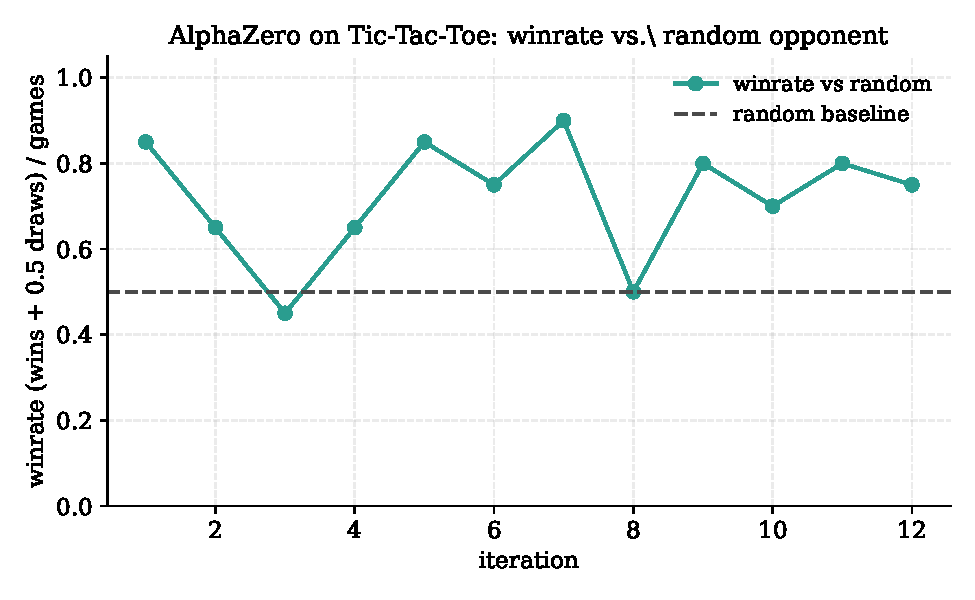
\includegraphics[width=0.85\linewidth]{figs/fig_az_winrate.pdf}
\caption{AlphaZero winrate vs.\ a uniform-random opponent on Tic-Tac-Toe.
The network is a tiny CNN (32 hidden conv channels) trained for 12
iterations of 5 self-play episodes with 25 MCTS simulations per move.
Winrate climbs from $\sim$0.5 (random) to $\sim$0.9 (almost-always wins
or draws against random). Note: against an optimal opponent, perfect play
on TTT yields a draw.}
\label{fig:az_winrate}
\end{figure}

\begin{figure}[h]
\centering
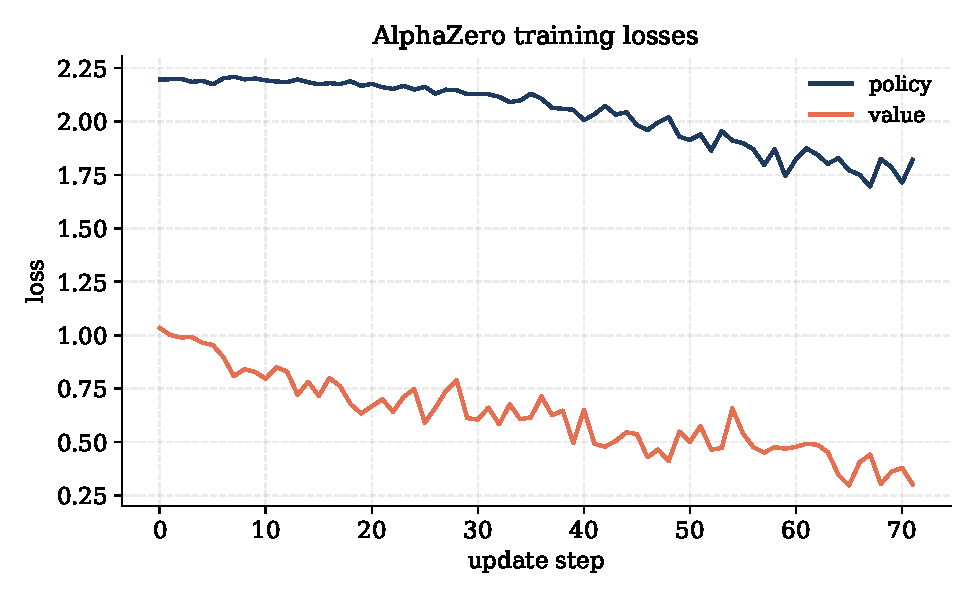
\includegraphics[width=0.85\linewidth]{figs/fig_az_losses.pdf}
\caption{AlphaZero training losses (policy CE + value MSE). Both decrease
smoothly; the value loss plateaus once the network has memorised the
terminal-value targets.}
\label{fig:az_loss}
\end{figure}

\begin{figure}[h]
\centering
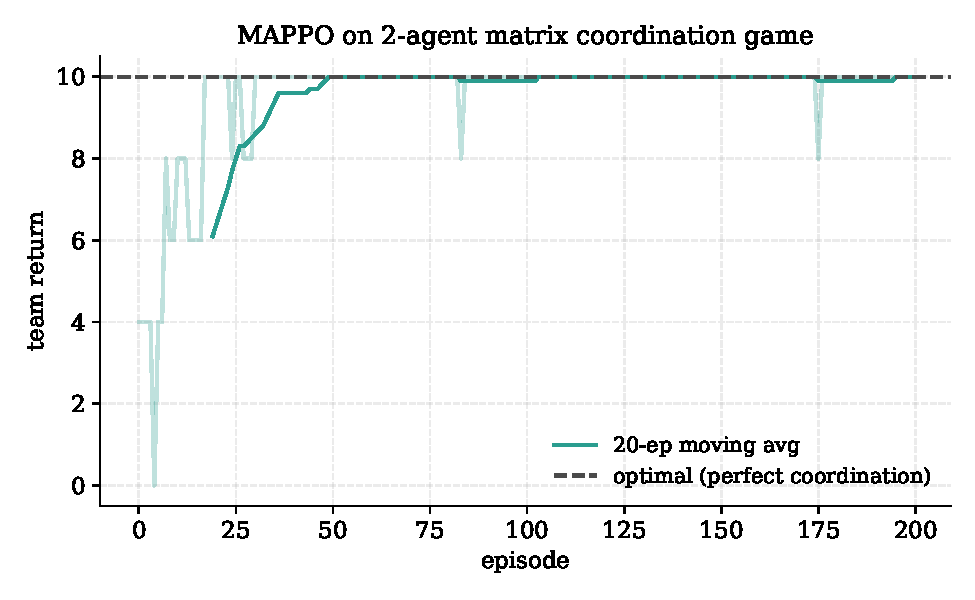
\includegraphics[width=0.85\linewidth]{figs/fig_coord_game.pdf}
\caption{MAPPO on a 2-agent matrix coordination game (3 actions, 5-step
episodes). Mean team return climbs to 10 (perfect coordination on every
step) in $\sim$200 episodes.}
\label{fig:coord}
\end{figure}

\begin{figure}[h]
\centering
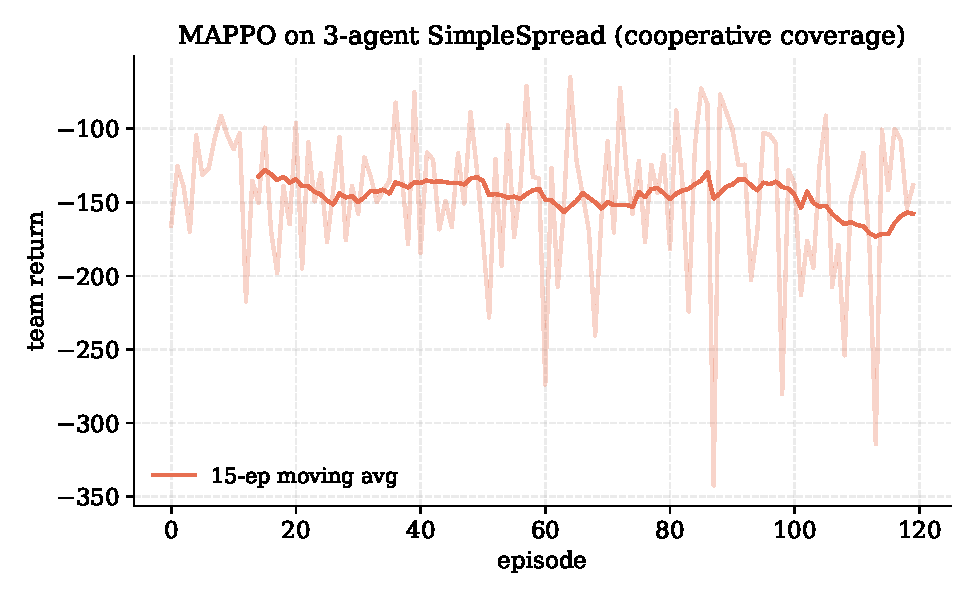
\includegraphics[width=0.85\linewidth]{figs/fig_simple_spread.pdf}
\caption{MAPPO on the 3-agent SimpleSpread cooperative-coverage problem.
Return is noisy because of random initial agent / landmark placements;
the moving-average curve shows mild improvement over 120 episodes.
Published SimpleSpread benchmarks need $\sim 10^4$ episodes for full
convergence; the figure is a snapshot of early learning.}
\label{fig:ss}
\end{figure}

\begin{figure}[h]
\centering
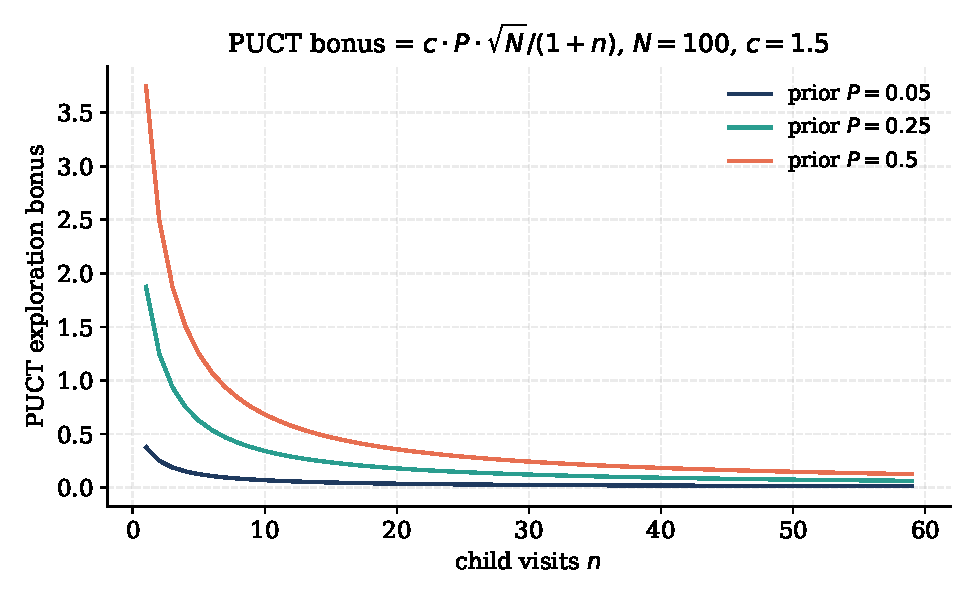
\includegraphics[width=0.8\linewidth]{figs/fig_puct.pdf}
\caption{PUCT exploration bonus as a function of child visits, for three
prior probabilities.}
\label{fig:puct}
\end{figure}

% =============================================================================
\chapter{Safety angle}

\begin{safetyangle}
Self-play and MARL fail in characteristic ways:

\textbf{F1 --- Policy collapse.} Self-play without Dirichlet noise (or
similar exploration) converges to a degenerate fixed point where the
network plays the same move regardless of state. \emph{Mitigation:}
Dirichlet noise at root (canonical AZ recipe); regular evaluation against
a fixed test opponent; reject training updates that collapse the policy
entropy below a threshold.

\textbf{F2 --- Cycle dynamics in general-sum MARL.} In games without a
unique Nash equilibrium (Rock-Paper-Scissors generalisations, cyclic
adversarial dynamics), naive multi-agent learning cycles among the cycle
of best responses without converging. \emph{Mitigation:} fictitious play
(average over historical opponent strategies, not just the latest);
PSRO; explicit exploration regularisation.

\textbf{F3 --- Cooperative coordination failure.} Multiple equivalent
Nash equilibria with incompatible actions (canonical example: two cars
at a 4-way stop --- both go = crash, both stop = deadlock). Without
explicit communication or a tie-breaking convention, agents may converge
to a coordination-failure equilibrium. \emph{Mitigation:} parameter
sharing (force agents to use the same network --- they cannot disagree
on the equilibrium they target); explicit communication channels;
Schelling-style focal points.

\textbf{F4 --- Reward hacking via opponent modelling.} In zero-sum
settings the agent may learn to exploit a specific opponent's
weaknesses rather than play robustly. The deployed system loses to
opponents not in the training distribution. \emph{Mitigation:} train
against a diverse opponent population (PSRO is exactly this); evaluate
against held-out opponents; use league training (AlphaStar) with
explicit ``main exploiters'' and ``league exploiters''.

\textbf{F5 --- Manipulating the centralised critic.} If the centralised
critic uses information unavailable at deployment, the deployed policy
may be much weaker than the training policy (because the actor was
trained against advantages it could not estimate from local
observations alone). \emph{Mitigation:} ablate the critic's
extra-information channels at training time periodically; ensure the
actor's policy is consistent with what a local-observation-only
estimator could rationalise.

Two cites: Vinyals et al., \emph{Grandmaster level in StarCraft II using
multi-agent reinforcement learning}, Nature 2019 (AlphaStar league
training); Schulman et al., \emph{Proximal Policy Optimisation Algorithms},
arXiv:1707.06347 (PPO that underpins MAPPO).
\end{safetyangle}

% =============================================================================
\chapter{Matching application}

\begin{matching}
Multi-agent and game-theoretic primitives apply to synthetic insurance / ATS in three
distinct places:

\textbf{Two-sided learning dynamics.} synthetic insurance is a multi-agent system: the
platform learns to allocate; the brokers learn to bid / archive. The
allocation policy and the broker strategy co-evolve. A naive ``platform
optimises bind rate'' policy plays into a general-sum game where brokers
adapt their book of business and bidding to what the platform rewards.
The Liu--Mania--Jordan AISTATS 2020 framework (Week 12) is the rigorous
version of this dynamic; PSRO is the algorithmic recipe for converging
to a stable equilibrium.

\textbf{Self-play for synthetic data}. When real labels are scarce
(early-stage synthetic insurance or a new ATS vertical), we can build a synthetic
adversary that generates challenging leads, and train the allocator
against it via self-play. AlphaZero-style policy iteration generates
both the data and the learner; the value head can be used as a
calibrated outcome predictor.

\textbf{Centralised training, decentralised execution.} The synthetic insurance panel
of brokers each runs their own scoring model (a recruiter desk runs its
own shortlist policy). A CTDE-style architecture --- a centralised value
function during training that consumes the joint allocator + broker
state, decentralised per-broker actors that consume only local
information --- is the right framework when brokers / recruiters have
heterogeneous information.

\textbf{Capstone connection (Week 24).} The capstone safety-aware
matching pipeline combines this week's CTDE machinery (centralised
critic with full information for training stability) with Week 11's OPE
(off-policy evaluation against the historical allocator), Week 12's
fairness LP (post-processor), and Week 22's CMDP (constrained MDP for
``never violate exposure floors''). The synthesis is the deliverable
of Week 24.
\end{matching}

% =============================================================================
\chapter{Exercises}

10 graded exercises (full statements in \texttt{workbook.ipynb}):

\begin{itemize}\setlength\itemsep{2pt}
  \item \textbf{E1} ($\star$) PUCT formula.
  \item \textbf{E2} ($\star$) Tic-Tac-Toe terminal value.
  \item \textbf{E3} ($\star$) Enumerate the 8 $D_4$ symmetries.
  \item \textbf{E4} ($\star\star$) Run MCTS for 30 simulations from the
        empty board; inspect the visit distribution.
  \item \textbf{E5} ($\star\star$) Train AlphaZero for 5--8 iterations; report
        winrate vs random.
  \item \textbf{E6} ($\star\star$) Implement GAE; verify on a simple sequence.
  \item \textbf{E7} ($\star\star$) Train MAPPO on the coordination game; verify
        convergence to 10/10.
  \item \textbf{E8} ($\star\star$) Train MAPPO on SimpleSpread; observe the
        learning curve.
  \item \textbf{E9} ($\star\star\star$, open-ended) Compare self-play
        vs.\ ``train against a fixed weak opponent''; argue why self-play
        produces stronger play.
  \item \textbf{E10} ($\star\star\star$, open-ended) AlphaZero ``ELO
        climb'': track winrate over iterations.
\end{itemize}

% =============================================================================
\chapter{Further reading}

The \texttt{extended\_reading.pdf} document covers five papers: Silver
et al.\ Nature 2017 (AlphaGo Zero), Silver et al.\ Science 2018
(AlphaZero), Yu et al.\ NeurIPS 2022 (MAPPO), Rashid et al.\ ICML 2018
(QMIX), Lanctot et al.\ NeurIPS 2017 (PSRO). Plus Vinyals et al.\ Nature
2019 (AlphaStar) and Schrittwieser et al.\ Nature 2020 (MuZero) as
bonus.

\emph{Sourced from} \texttt{research/deeprl\_core\_sota.md} sections
covering MARL and self-play.

\end{document}
